\documentclass[11pt]{article}
%\documentclass[11pt,oneside,openany]{book}
%\usepackage[margin=1in]{geometry}
%\usepackage{prelude}

\usepackage[hyphens]{url}
\usepackage[implicit=true,%
            bookmarks=false,%
            bookmarksopen=false,%
            pdfpagemode=UseNone,%
            pageanchor=false,
            colorlinks=false,%
            pdfborder={0 0 0},%
            plainpages=false,%
            pdfpagelabels=true,%
            pdfpagelayout=SinglePage]{hyperref}
\usepackage[sort&compress,numbers]{natbib}
\usepackage{skull}
\usepackage{ragged2e}
\usepackage{fancyhdr}
\usepackage{xspace}
\usepackage{fullpage}
\usepackage{graphicx}
\usepackage[capitalize,sort&compress]{cleveref}
\usepackage{mathptmx}
\usepackage[scaled=0.83]{berasans}
\usepackage[scaled=0.83]{beramono}
\usepackage[colorinlistoftodos]{todonotes}
\usepackage{alltt}
\usepackage[OMS,OML,T1]{fontenc}
\usepackage{textcomp}
\usepackage{caption}
\usepackage{subcaption}
\usepackage{paralist}
\usepackage{wrapfig}

\usepackage{setspace}
%\singlespacing

\newcommand{\reffig}[1]{Figure~\ref{#1}}
\newcommand{\refsec}[1]{Section~\ref{#1}}


\renewcommand{\bfdefault}{b} % used to eliminate most
\renewcommand{\sldefault}{it} % "font not found" warnings
\usepackage{tikz}
\usetikzlibrary[backgrounds,calc,positioning]
\usepackage{enumitem}

\begin{document}

\author{Hannah Quay-de la Vallee}
\title{By the People, For the People: \\ Community Ratings of App Privacy \\ \ \\ Thesis Proposal}
\date{May 19, 2015}

\maketitle

\maketitle % PROPOSAL

\newpage

\tableofcontents % PROPOSAL

\newpage

\doublespacing


\setcounter{page}{1}
\pagestyle{empty}
\hypersetup{pageanchor=false}


\pagestyle{plain}

\begin{abstract}

Apps use access to hardware resources and sensitive 
user data to enable users to customize their devices. 
Because these apps are usually written by untrusted 
third-parties, they become significant attack vectors 
on users' security and privacy. To protect themselves, 
users need to be able to control apps' access to 
sensitive resources. Most systems thus give users 
the impression of control by requiring some form of 
consent, such as the install-time permissions on Android. 
Unfortunately, many users lack the 
information and expertise needed to make informed 
decisions. The proliferation of app stores beyond 
phones and browsers to cars, watches, and more will 
only exacerbate this problem. 

I propose a marketplace that employs user ratings for 
app permissions as a mechanism to inform users about 
the potential risks of these permissions. This allows 
users with opinions and concerns about app permissions 
to share their views with other users. This thesis will 
design and build such a marketplace. It will use 
crowdsourcing to validate the interface design and it will
gather and compare permission ratings from a variety of 
sources (such as crowd workers, college students, security 
experts, and automated systems). It will investigate how to customize 
the marketplace to make it better suited to each user. 

Along with building the marketplace, this thesis will 
also examine how user ratings can help users make better 
selections and assist developers in meeting user needs.

\end{abstract}



\doublespacing


\section{Introduction}

\emph{\paragraph{Thesis Statement}
Ratings of apps' privacy, in addition to ratings of functionality, 
can enable an app marketplace that incorporates user privacy into 
the app ranking process.}

Apps have become pervasive
in consumers' lives 
\cite{gplay-50-billion, apple-50-billion}.
Most commonly associated with smartphones and tablets, 
such as iPhones, iPads and Android devices, the app model now has much 
wider adoption, appearing in a variety of domains,
such as browsers (in the form of extensions), PC operating 
systems, smartwatches (such as the Pebble and the Apple Watch), 
home automation,
and cars.
%TODO: New citations (like Microsoft's HomeOS \cite{ms-homeos}) 
%(such as \emph{iOS in the Car} \cite{cars-apple} and Android's 
%partnership with Audi, GM, and Honda \cite{cars-google}).
Most app ecosystems are supported by a store or
\emph{marketplace}---a central repository that
enables users to search for, browse,
investigate, and install apps on their devices. 

Apps and app stores allow users of a broad range
of technical ability to customize their devices.
However,  
because of the amount of user information associated with these 
devices, installing third-party apps presents 
risks to user security and privacy. Some of these risks are malware apps or 
apps that highjack legitimate apps
to perform malicious operations. These problems are the topic
of extensive research 
\cite{droidrisk-2013, android-repackaged-CODASPY12, comDroid-MOBISYS11}, 
%TODO: Update citations
but that research does not address a different,
important problem: How can systems help users make informed privacy and
  security decisions about apps based on the permissions that the apps
  require?
In this thesis, I will demonstrate that \emph{ratings of app 
privacy can enable an app marketplace that incorporates user 
privacy into the app ranking process.} This could help users 
find apps that align with their privacy needs.

Many app platforms currently try address the issue of
user privacy by controlling apps' access to hardware resources 
and user data with some type of permissions system,
and require user consent before an app can use any
of those resources and data. Permission models and their presentation 
vary across operating systems. Take, for example, the permission systems
for Android and iOS, the two most popular smartphone operating systems.  
Android takes a ``static'' approach, in that apps are given a
\emph{manifest} of
permissions at installation time, and may use any of them at will at runtime.
Users must approve these during the installation
process. In contrast, iOS uses a ``dynamic''
approach: permissions are not listed approved up-front; instead, users must
approve access to permissions as an app tries to use them.

There are advantages and disadvantages to each approach, but
this proposal will use the static model. For one thing, only in 
knowing all permissions can users reason about their potential
combinations. Furthermore, I believe that asking for permissions
during execution will often result in consent that might not otherwise
have been given, because users are likely to grant whatever appears
necessary to complete a the task at hand \cite{phisher-wanings-SIGCHI08}. 
In contrast, the static
model, in principle, enables a more contemplative and
informed approach to choosing apps based on permissions.

In theory, requiring users to approve permissions gives them control over their 
data, but in practice users often do not have the 
information or expertise to meaningfully consent to an 
app's required permissions. Users may not
know why the given app requires a certain permission, or
even what it means \cite{android-attention-SOUPS12}. 
Context is critical:
for instance, 
a ``share with social media'' permission is necessary for a social
networking app but may be utterly
unsuitable for a medical monitoring app. 
For those users who do have opinions about permissions, 
there is no structured method to
communicate their thoughts---comments to this effect are often found in
the ratings of apps, but these comments can be difficult for other
users (especially uninformed ones who would like guidance), and even
developers, to find. In turn, developers have no structured way to
respond to such comments and justify their apps' needs.
%\footnote{Sometimes, 
%seemingly unnecessary permissions can appear to have justifications. 
%TODO: How do I reference SK here?
%For instance, the I communicated
%  with the developers of Dropbox, asking why it needed ``Phone calls
%  -- read phone state and identity''. Their response was, ``[T]he
%  phone state \& identity is simply because we need a unique ID for
%  each cell phone, so we use the IMEI to keep track of phone/user
%  combinations.'' This arguably points to a weakness of the Android
%  APIs, which others have noted \cite{effectivness-perms-USENIX11}
%  \cite{septa-perm-explain}.} Finally, this entire problem
%is greatly exacerbated by continuously growing manifests.

I am building a crowdsourced app marketplace that allows users to review
each of an app's individual \emph{permissions}, rather than just the app's functionality. 
It also allows developers to
explain why they requested a permission---sometimes due to the
weaknesses of a permission model, such as excessively coarse permissions
\cite{permission-tracking-UBICOMM12}---and how they intend to use it. This both enables more
informed user decisions and creates accountability of a developer's intent.


%This would allow users to communicate in a structured way with one
%another and with developers. These dialogues can spur developers to 
%adjust their app's permissions to better meet uses' need.
%An incident with Avis illustrates a (sadly,
%rare) success. Avis added ``List of Running Apps'' to the permissions
%required by their Android app. Users protested the change in the
%reviews, with numerous comments such as, ``I refuse to update and will
%likely uninstall until you can justify the need to access my `Running
%Apps'.'' In response to the backlash, Avis removed the offending
%permission in later versions of the app. Avis explained the removal on their app's Google Play
%page, stating:
%\begin{quote}
%  We've updated the permissions in this version to not require List of
%  Running Apps. We had that in place to help analyze and improve app
%  performance, but removed it due to your voiced concerns.
%\end{quote}

%My goal is to make such successes commonplace. I intend to leverage
%the willingness people already demonstrate to provide ratings, and
%their familiarity with mechanisms like rating systems, by building systems to rate
%\emph{permissions}. These ratings then serve as a guidepost to other
%users as they choose which apps to install. 
%Indeed, the ratings can be used to \emph{rank} apps
%so that more privacy-sensitive apps are rewarded by appearing higher,
%while questionable ones percolate down in the list. In turn, a
%permission-rating app interface becomes a channel for developers to
%convey their needs and intent back to users, thereby enabling more
%informed decisions. The feedback of developers also documents their
%intent, which can be cross-checked by other tools (e.g., program
%analyses).

\section{Preparatory Work}
\label{sec-prep-work}

My goal is to build a marketplace that employs user-provided 
ratings to sort apps, and displays these ratings to other users 
to assist them in their app selection process. For such a marketplace
to be useful, it would need a couple of things:  it must have
user ratings, and it must present those ratings to users in
an easy-to-understand way. In Sec~\ref{subsec-seeding} I will 
discuss how to gather ratings to seed the marketplace so that 
it can be immediately useful to users, and in Sec~\ref{subsec-perm-ui}
I will show how I designed an interface to present these ratings 
to end users. I will discuss future work on the marketplace in 
Sec~\ref{subsec-the-apps}.

\subsection{Seeding the Marketplace}
\label{subsec-seeding}
Because the marketplace relies on user ratings, it presents 
a chicken-or-egg problem: In order to get users
to employ systems that show ratings, there must already be present
ratings that offer some value to the user; but users would have to be
using a rating app already in order for it to collect user
ratings. I therefore wanted to investigate other ways to
acquire ratings for the marketplace.

Because I would prefer to have a large number of ratings,
crowdsourcing seemed a natural fit. However, crowdsourcing via
platforms like Amazon's Mechanical Turk also raises various concerns. Will
reviewers take the rating task seriously? Will they give ratings that
are actually distinct enough to reveal differences? Will they rate the
permissions in the context of a given app? This last point is subtle: permissions are
not inherently ``good'' or ``bad'', but acquire meaning in the context
of the app's intended purpose.\footnote{For example, my advisor
  downloaded an app that helped turn on and off individual permissions
  on the basis of perceived threat. However, the threat was not
  specific to the app. Thus, on the very first app he examined---that
  for Google+---the permission marked as most dangerous was that to
  share to social streams\dots which is the very point of the app.}

Based on these concerns, I did a series of preliminary studies designed to answer
these questions:
\begin{itemize}
\item Could I gather a large number of conscientious ratings through crowdsourcing?
\item Would those ratings be useful?
\item What are some factors that might affect how users perceive and rate 
app permissions?
\end{itemize}
I deployed a series of studies on Mechanical Turk. I chose
Mechanical Turk because it can be cost effective, and has become
a common platform for academic research, which provided a body of work on how
to best use it \cite{reseach-mturk-BRM12, mturk-data-quality-PPS11}. 
My study presented subjects with surveys that
described an app, preceded by a motivating paragraph asking
them to imagine that they came by this app in some way and needed an
app of that functionality.  I used fourteen apps: Facebook, GMail,
Pandora, Angry Birds and ten weather apps.  The descriptions
of the apps were taken from their Google Play pages, including the
permission information. Given this information, users were asked
whether they would download the app, and to rate each of the app's
permissions as either ``acceptable'' or ``unacceptable,'' and were
given an optional text box to explain each of their ratings.

Once I had subjects completing tasks, I needed to ensure that they 
were real humans who were actually answering the questions I
asked. I manually reviewed the responses from the text boxes
that allowed users to explain their ratings. Overall, I found that
many subjects did provide explanations for their ratings despite this being
optional. Furthermore, their responses were relevant to the
permissions being discussed, indicating that the responses were from
real people thinking about the task. Because these were preliminary
studies, I did not do any significant analysis on the text answers,
but I will in proposed work. Additionally, I will want to further
validate my Mechanical Turk results by comparing them with results
from other populations such as students and security experts. 
There are also other measures I will
use to increase confidence in my Mechanical Turk data, such as test
questions (like ``which Android phone do you have?'').

\begin{figure*}[t]
\centering
    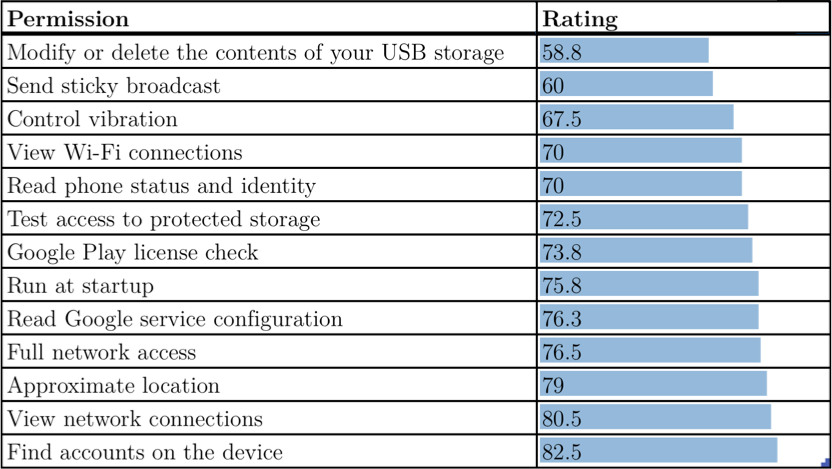
\includegraphics[width=.6\linewidth]{img/RatingTable.png}
    \vspace{1pt}
    \caption{The range of approval ratings for the permissions from the 
    weather apps surveyed}
    \label{weatherratings}
\end{figure*}

Next, I looked for variations in ratings between permissions. To
compare within a domain, I focused on the weather apps. Across the
ten apps, a total of thirteen permissions were used. These were rated
as shown in Fig.~\ref{weatherratings}.  Although the approval rate for
every permission was over 50\%, approval varied from 58.8\% to
82.5\%. The range of ratings suggests that users were actually
distinguishing between the permissions (not treating them all
uniformly, which might be another indication of not taking the rating
task seriously or not understanding it); I also found correspondence
between their ratings and their textual comments.

To investigate factors that might affect user ratings, I looked only at Facebook, Gmail,
Pandora, and Angry Birds.  I used the same basic surveys, but
varied specific conditions in the survey. The conditions 
were: asking half the subjects if they would download the app before 
they were asked to rate the permissions and asking the other half after; 
varying how the subject supposedly discovered the
app (on recommendation from a colleague, because it was a featured app in
the app store, or because it was highly rated in the app store); and
varying whether the app was ``brand-name'' or generic. To create the generic
apps, I reused the Play Store descriptions of the apps but replaced all
instances of the app's name with a generic name. For example, GMail
became MongogoMail.  Additionally, I changed any obvious identifiers,
so the pigs and birds from Angry Birds became warriors and invaders.

Varying where subjects were asked whether they would download the app 
(either before or after rating the permissions) was
meant to investigate whether users were more or less likely to
download an app if they had been primed to think about privacy by
rating the permissions. I found that there was no significant change
in either the percentage of subjects who would download the apps, or the
ratings the provided.

Varying how the subject was asked to imagine they discovered the app
could affect their opinion of the permissions, or their willingness to
download the app. In this case, only Facebook showed any interesting
results: respondents were less likely to install the app if it
had been recommended by a colleague than if it was featured or highly
rated. I found this result is odd given that, due to the network
effect of an app like Facebook, I would expect the app to be more
valuable if friends or colleagues also use it. However, it did not
seem to be a pervasive effect.

Varying branding did not have a significant effect on downloads or
ratings for Pandora and Angry Birds, but did 
for GMail and Facebook. In both cases,
participants rated the generic version's permissions as less
acceptable. However, for GMail, a lower percentage of users said they
would install the app, but this was not true of Facebook.  These
findings suggest that branding may be an important part of users'
feelings about an app. However, these results also raise questions
about how privacy and functionality interact in user decisions. Are
people less approving of these generic apps because they think they
are unsafe, or is their perception of the app altered because they 
feel they will not have access to their
existing email and social network accounts, 
and so don't see the permissions as worth the risk?

To separate access concerns from privacy concerns, I did a follow-up
study asking subjects to evaluate an app that was an
interface over a brand-name app. For instance,
subjects were presented with Gmore!, an app purporting to offer a
smoother interaction with one's GMail account. Again, subjects rated
the off-brand apps' permissions as less acceptable, and again, a lower
percentage of users said they would use Gmore!. This suggests that
subjects were concerned about the privacy of the apps, not just their
functionality.

My preliminary studies suggest that I will be able to gather
meaningful ratings from Mechanical Turk. I believe this is vital
to seed data in a privacy-centric marketplace, and hence attract users
to it. Further, my early examination of these ratings 
suggests insights into how users think about their privacy, and reveals
factors that affect their opinions. These insights may be useful for
further development of my marketplace, and may also be more broadly
useful to the privacy research community.

\subsection{The Permission User Interface}
\label{subsec-perm-ui}

Because I want to communicate rating information to users,
the interface for displaying the ratings is another critical component of 
my system. The interface should help users understand the 
riskiness of individual permissions so they can make \emph{informed}
decisions without requiring significant
effort. Ideally, it would be 
intuitive enough that users could understand it without too 
much direction. \reffig{grade-perms} is an example of what such an interface
might look like.

Designing such an interface proved surprisingly subtle. 
My original designs, based on existing security 
metaphors, failed to convey the desired information.
Indeed, I found that some of them \emph{actively 
mislead users} (\refsec{sec-ui-design}).
I also unearthed some common patterns of interface
confusion. In the end I found three designs that appear to work, and
conducted a large user study to confirm this
(\refsec{s-sec-largescale}). One of these designs will be used in the new
marketplace.

\subsubsection{Exploratory Interface Design}
\label{sec-ui-design}

To find a functional interface, I designed several prototypes and 
leveraged Amazon's Mechanical Turk platform to give me rapid feedback 
on those prototypes.

\paragraph{Methodology}
\label{subsec-small-methods}

\begin{wrapfigure}{l}{0.5\textwidth}
    \begin{center}
        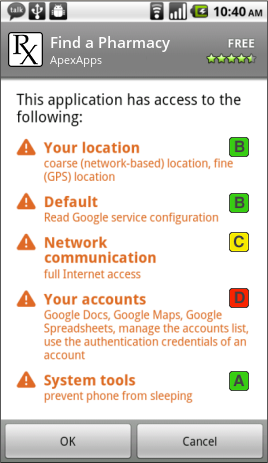
\includegraphics[width=.8\linewidth]{img/GradesPerms.png}
    \end{center}
    \caption{A prototype interface for permission ratings.}
    \label{grade-perms}
\end{wrapfigure}

I explored each prototype with a survey on Mechanical Turk.
These surveys were 
intended to expose broad conceptual problems 
in the interfaces, so I recruited only 10 to 12 
subjects per interface. The surveys focused on two issues: how well subjects 
understood the purpose and meaning of the interface absent any explanation, 
and whether subjects understood where the ratings came from.

During each study, subjects were shown a mock-up of
a candidate interface. \reffig{grade-perms}
is an example of such a mock-up. The mock-ups displayed the full permissions
interface for a fictional app called Find a Pharmacy, which appeared 
to be developed by the (also fictional) company ApexApps. 
I chose a pharmacy locator app because it 
could pose a privacy risk to a user (if, for example, it stored a list
of the user's medications for refill reminders), but 
would be unlikely to offend any 
subjects. Each mock-up used different iconography to
present the user permission ratings (which were also fake), but the permissions
and their rating values were the same or comparable across interfaces. 

The mock-ups were presented as static images that were tall enough
not to require scrolling. (Because the rating icons
varied in size, the mock-ups varied in height.) This was both
to ensure subjects did not miss any of the iconography by failing to
scroll, and to avoid distraction induced by interaction.

Upon being presented with one of the mock-ups, subjects were
asked to explain, in a free-response text box, 
what they thought the icons next to the permissions 
meant. Subjects were given no information about the 
purpose of the interface. The next page of the survey 
told them that the icons were privacy 
ratings and asked them to rate how clear this was from 
the interface, on a 4-point Likert-type scale. 

I manually examined 
the text responses to identify conceptual problems with each 
interface, whereupon I either attempted 
to redesign the interface to address issues raised by subjects, 
or I decided the interface was not viable and disqualified it.
Using this process I eliminated all but three interfaces, which I evaluated
in a larger study (\refsec{s-sec-largescale}).

To understand subjects' beliefs about the ratings' source, I asked
whether they thought the ratings came from 
 ``other Android users'', ``independent 
security experts'', ``a review team at Google'', or
``don't know''. I discuss the outcome of this question
before delving into the individual interfaces.


\paragraph{The Source of the Ratings}
\label{subsec-small-source}

If users are going to trust the ratings enough to use them, 
they are placing trust in the raters, so it is
important that users understand the \emph{source}
of the ratings. 
I found that most of the interfaces failed to
convey to subjects that the ratings were from other Android users.
This is therefore something that should be considered in the 
design of the complete marketplace.

\label{ss-sec-stars-r1}
\begin{wrapfigure}{l}{0.5\textwidth}
\begin{center}
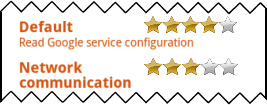
\includegraphics[width=.9\linewidth]{candidate-img/stars/starsR1.png}
\end{center}
\end{wrapfigure}

\paragraph{Stars}
\label{s-sec-stars}

A five-star system is possibly the most common iconography for user ratings,
and is already in use in the Google Play store to display apps' overall 
functionality ratings. It is therefore a natural basis for experimentation.

% \,\protect\includegraphics[height=10pt]{img/TinyStars.png}}


Possibly due to the ubiquity of five-star ratings, 
subjects seemed to have preconceptions 
about the meaning and source of the ratings. This proved to be both an 
advantage and a disadvantage. On the positive side, 
subjects correctly understood the source of
the ratings (other Android users), and that more stars corresponded to a 
better rating.

Unfortunately, subjects' association with stars as a \emph{functionality} rating 
was \emph{too} strong. Many subjects thought the ratings indicated how well 
the permissions' services worked. For example, some subjects thought the rating next 
to ``Network Communication'' showed the strength of the network signal. 

In order for the star ratings to effectively communicate the meaning of the permission 
ratings, users would have to understand that the same icon
on the same page had two different meanings (the app's functionality
rating and the permission ratings). This potential for user confusion led
us to eliminate this interface.
However, it did inspire interfaces using privacy-relevant symbols rather than stars, with 
the intention of
leveraging users' existing understanding of an out-of-five system while
expressing that the ratings are about privacy.


\begin{wrapfigure}{l}{0.5\textwidth}
\begin{center}
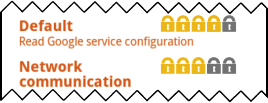
\includegraphics[width=.9\linewidth]{candidate-img/locks/locksR1.png}
\end{center}
\end{wrapfigure}

\paragraph{Locks}
\label{s-sec-locks}

One symbol I used place of stars was locks, a natural visual metaphor for protection.
My original lock design used yellow locks over a grey background:
% \,\protect\includegraphics[height=10pt]{img/TinyLock1.png}}
%\label{ss-sec-locks-r1}
%\begin{center}
%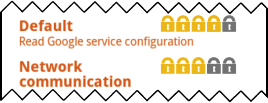
\includegraphics[width=.5\linewidth]{candidate-img/locks/locksR1.png}
%\end{center}
This design caused a number of
misconceptions.
First, although most subjects understood that the locks were privacy 
ratings, some thought they meant that 
the permission's service was restricted. (This may 
stem from the practice by developers of using locks to mark features of 
an app that must be purchased or earned before they can be used.)
Second, those subjects who \emph{did} understand that the locks represented privacy ratings
could not tell whether more yellow locks denoted a better or worse 
rating. This is troubling, because it would cause users to think the most 
dangerous permissions were the safest. I label this confusion,
present in many interfaces, the 
\emph{better-or-worse} phenomenon, and discuss it more in \refsec{common-findings}.

\begin{wrapfigure}{r}{0.5\textwidth}
\begin{center}
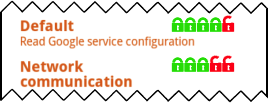
\includegraphics[width=.9\linewidth]{candidate-img/locks/locksR2.png}
\end{center}
\end{wrapfigure}

The second lock interface, drawing from the traffic light interface
(\refsec{ss-sec-traffic-r2}), tried to eliminate the better-or-worse 
phenomenon by using red and green locks:\footnote{For this 
  study, I chose colors
  compatible with red-green colorblindness, but any deployed system
  should address the full spectrum of colorblindness.}
% \,\protect\includegraphics[height=11pt]{img/TinyLock2.png}}
\label{ss-sec-locks-r2}
%\begin{center}
%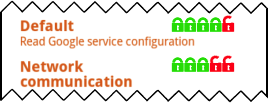
\includegraphics[width=.5\linewidth]{candidate-img/locks/locksR2.png}
%\end{center}
To further reinforce the message of privacy, the 
green locks were closed and the red locks open.
I also hoped that using color would reduce 
the perception that the locks indicated restricted services (in which 
case \emph{fewer} locks would be preferable).
Though these changes helped curtail the better-or-worse phenomenon, they did not 
eliminate it entirely. 


\begin{wrapfigure}{l}{0.5\textwidth}
\begin{center}
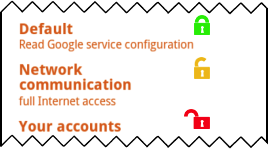
\includegraphics[width=.9\linewidth]{candidate-img/locks/locksR3.png}
\end{center}
\end{wrapfigure}

Because the better-or-worse phenomenon was at least partially caused 
by confusion about whether more or fewer icons was better, I 
replaced the out-of-five system with 
a single lock next each permission, and relied on 
color and open-ness to convey the rating:
% \,\protect\includegraphics[height=10pt]{img/TinyLockGreen.png}\,
%\protect\includegraphics[height=10pt]{img/TinyLockYellow.png}
%\protect\includegraphics[height=10pt]{img/TinyLockRed.png}}
\label{ss-sec-locks-r3}
%\begin{center}
%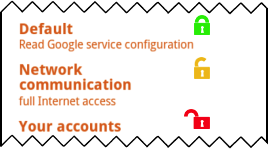
\includegraphics[width=.5\linewidth]{candidate-img/locks/locksR3.png}
%\end{center}
Using
only red and green locks would have been too similar to the checkbox
interface (see \refsec{ss-sec-binary-r1}), 
which had resulted in dangerous misunderstandings by subjects. 
To avoid this, the interface also used half-open yellow 
locks. This 
had the added benefit of conveying more 
information than just red and green locks without adding much cognitive 
effort.

\begin{wrapfigure}{r}{0.5\textwidth}
\begin{center}
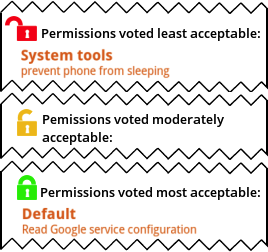
\includegraphics[width=.9\linewidth]{candidate-img/locks/locksR4.png}
\end{center}
\end{wrapfigure}

This redesign improved understanding, but 
some subjects still thought that the locks indicated inaccessible features.
To further clarify the icons' meaning, I grouped 
permissions by rating and added explanatory 
text alongside the icons, drawing 
from the design of the first traffic light interface 
(\refsec{ss-sec-traffic-r2}).
(Additionally, I hoped introducing the word ``voted'' 
would also clarify the source of the ratings by emphasizing that they 
were an aggregate of community opinions.)
% \,\protect\includegraphics[height=10pt]{img/SmallLockGreen.png}\,
%\protect\includegraphics[height=10pt]{img/SmallLockYellow.png}
%\protect\includegraphics[height=10pt]{img/SmallLockRed.png}}
\label{ss-sec-locks-r4}
%\begin{center}
%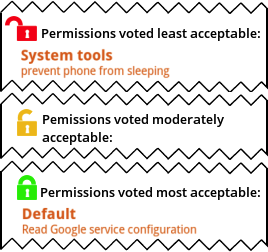
\includegraphics[width=.5\linewidth]{candidate-img/locks/locksR4.png}
%\end{center}
The final lock interface was an improvement over its 
predecessors, 
but some subjects still thought the locks indicated 
availability. Since locks 
%The final lock interface was better than its 
%predecessors, but some subjects still thought the locks indicated 
%availability. Since locks 
performed worse than percentage bars (\refsec{ss-sec-pbars-r4}) 
and traffic signs (\refsec{ss-sec-traffic-r4}), 
I eliminated this interface family.


\begin{wrapfigure}{l}{0.5\textwidth}
\begin{center}
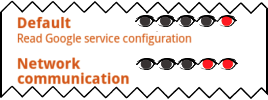
\includegraphics[width=.9\linewidth]{candidate-img/eyes/eyesR2.png}
\end{center}
\end{wrapfigure}

\paragraph{Eyes}
\label{s-sec-eyes}

Continuing my exploration of other symbols in an out-of-five rating, this 
interface used eyes in the place of stars. My first icon, which
used a no-smoking-style circle-and-slash over an eye, 
proved too difficult to see at small scale
(some subjects thought it was a watch). I thus tried different-color eyes:
\label{ss-sec-eyes-r2}
%\begin{center}
%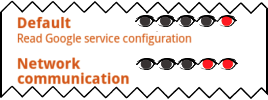
\includegraphics[width=.5\linewidth]{candidate-img/eyes/eyesR2.png}
%\end{center}
The more dangerous a permission was, the more red eyes it had; the more
benign it was, the more grey eyes it had.
Additionally, the red centers had 
the appearance of a red recording light as seen on a camera.

Though subjects could now see the icon, this interface exhibited 
the better-or-worse phenomenon. One possible cause is that 
the grey eyes looked more like actual eyes, and so subjects thought that more 
grey eyes meant more surveillance. 

I tried various redesigns such as grouping permissions by rating with a
text header (as 
in \refsec{ss-sec-locks-r4}) and introducing a yellow eye category. Though these changes helped, 
percentage bars (\refsec{ss-sec-pbars-r4}) and traffic signs 
(\refsec{ss-sec-traffic-r4}) were still better understood by subjects,
so I disqualified this interface.


\begin{wrapfigure}{l}{0.5\textwidth}
\begin{center}
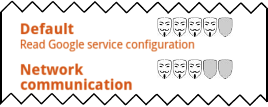
\includegraphics[width=.9\linewidth]{candidate-img/masks/masksR1.png}
\end{center}
\end{wrapfigure}

\paragraph{Guy Fawkes Masks}
\label{s-sec-masks}

I also explored out-of-five ratings using Guy Fawkes masks, which 
were popularized by the graphic novel \emph{V for Vendetta} and its
film adaptation, and have since become a symbol for personal
privacy and activism.
% \,\protect\includegraphics[height=12pt]{img/TinyMasks.png}}
\label{ss-sec-masks-r1}
%\begin{center}
%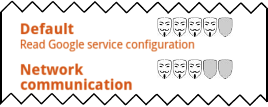
\includegraphics[width=.5\linewidth]{candidate-img/masks/masksR1.png}
%\end{center}
Unfortunately, subjects felt the
rating showed how well protected their information was from the government 
(possibly due to the ``hacktivist'' group Anonymous' adoption of the mask as a symbol). 
As this is not a protection a permissions system can provide and it is dangerous for an
interface to suggest protections that do not exist, I eliminated all
variations of this design.

\newpage

\begin{wrapfigure}{l}{0.5\textwidth}
\begin{center}
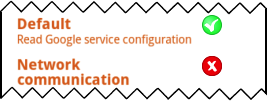
\includegraphics[width=.9\linewidth]{candidate-img/checkboxes/checkboxesR1.png}
\end{center}
\end{wrapfigure}

\paragraph{Binary Checkboxes}
\label{s-sec-checkbox}

As I wanted to convey information without demanding much cognitive effort,
I designed a simple interface in which 
each permission was given either a green 
checkmark indicating users approved of the permission or a red X indicating 
they did not approve.
% \,\protect\includegraphics[height=10pt]{img/TinyCheck.png}\,
%\protect\includegraphics[height=10pt]{img/TinyEx.png}}
\label{ss-sec-binary-r1}
%\begin{center}
%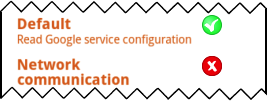
\includegraphics[width=.5\linewidth]{candidate-img/checkboxes/checkboxesR1.png}
%\end{center}
Unfortunately, I discovered a very significant confusion: in this interface
the red X was meant to indicate a potentially invasive permission, but 
subjects thought it meant that the given permission had been \emph{disabled}. This
is an extreme case of the better-or-worse phenomenon and is an 
alarming misconception. I therefore eliminated this interface without attempting to 
redesign it.


\begin{wrapfigure}{l}{0.5\textwidth}
\begin{center}
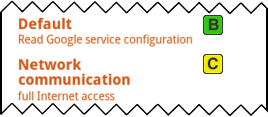
\includegraphics[width=.9\linewidth]{candidate-img/grades/gradesR1.png}
\end{center}
\end{wrapfigure}

\paragraph{Grades}
\label{s-sec-grades}

Drawing on another iconography, this 
interface used letter grades to present the ratings. 
Typically used to rate students' academic performance, 
grades are also used in some non-educational settings (e.g., 
the New York City Department of Health restaurant 
inspection results).
% \,\protect\includegraphics[height=10pt]{img/A.png}\,
%\protect\includegraphics[height=10pt]{img/C.png}\,
%\protect\includegraphics[height=10pt]{img/D.png}}
\label{ss-sec-grades-r1}
%\begin{center}
%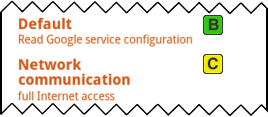
\includegraphics[width=.5\linewidth]{candidate-img/grades/gradesR1.png}
%\end{center}
Unfortunately, most subjects thought the ratings were for 
the functionality of a permission's service. As this interface failed
in its primary purpose, I eliminated it.


\begin{wrapfigure}{r}{0.5\textwidth}
\begin{center}
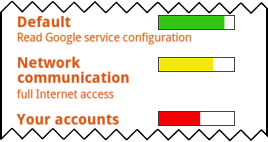
\includegraphics[width=.9\linewidth]{candidate-img/bars/barsR1.png}
\end{center}
\end{wrapfigure}

\paragraph{Percentage Bars}
\label{s-sec-pbars}

Eschewing existing privacy and safety metaphors,
this interface used rectangular bars to indicate 
the percentage of raters who considered a given permission to be acceptable.
This style of rating conveys more information than the other
interfaces, and therefore carries a greater risk of overwhelming a user. To mitigate this 
issue, the bars were colored red, yellow, or green depending on the permission's approval 
rating, giving a more obvious visual distinction between ratings:
% \,\protect\includegraphics[height=8pt]{img/Bars12/GreenWhiteBar.png}\,
%\protect\includegraphics[height=8pt]{img/Bars12/YellowWhiteBar.png}\,
%\protect
\includegraphics[height=8pt]{img/Bars12/RedWhiteBar.png}}
\label{ss-sec-pbars-r1}
%\begin{center}
%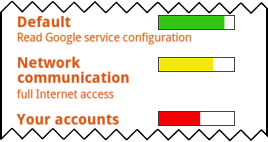
\includegraphics[width=.5\linewidth]{candidate-img/bars/barsR1.png}
%\end{center}
Subjects understood that the bars indicated privacy ratings, 
and this interface did not suffer from the better-or-worse
phenomenon, due in part to the colors of the bars. 
One subject stated the bars rated the permissions from ``most risky to the least, 
red being the highest and the green being generally safe''.

Although the bars were effective, subjects' feedback on 
the traffic signs interface (discussed below) 
revealed a potential pitfall: their comments suggested that subjects 
perceived a green light as a signal to proceed without caution, which could 
encourage users to download an app without considering the permissions at all. I 
was concerned the green bars 
could have the same over-soothing effect.

To encourage caution in all cases, I modified the interface to use 
red, orange, and yellow bars. This interface had 
two variations. In both, more dangerous permissions had red
bars and less dangerous permissions had yellow bars. In the first variant, the more 
dangerous a permission, the fuller its bar would be (showing the percentage of 
raters who deemed the permission \emph{unacceptable}). These bars might look like 
\includegraphics[height=8pt]{img/Bars3/RedBig/YellowWhiteBar.png}\,,

\includegraphics[height=8pt]{img/Bars3/RedBig/OrangeWhiteBar.png}\,, and 

\includegraphics[height=8pt]{img/Bars3/RedBig/RedWhiteBar.png}. In the second variation, the more
dangerous a permission, the more empty its bar (showing the percentage of raters who 
deemed the permission \emph{acceptable}). These bars would look like 
\includegraphics[height=8pt]{img/Bars3/RedSmall/YellowWhiteBar.png}\,,

\includegraphics[height=8pt]{img/Bars3/RedSmall/OrangeWhiteBar.png}\,, and

\includegraphics[height=8pt]{img/Bars3/RedSmall/RedWhiteBar.png}.

Both versions of this interface introduced the 
better-or-worse phenomenon. It is possible that,
because all of the colors were ``warning colors'', the effectiveness of the color 
differentiation was diminished. Additionally
these colors could cause warning fatigue after continuous use.


\begin{wrapfigure}{r}{0.55\textwidth}
\begin{center}
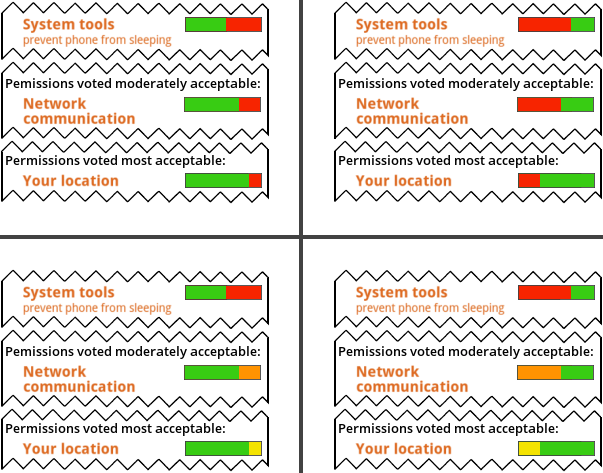
\includegraphics[width=.9\linewidth]{candidate-img/bars/barsR4.png}
\end{center}
\end{wrapfigure}

To avoid these problems, we
introduced two-color bars. As before, each bar had some percentage of 
a warning color, (the percentage of raters who deemed the permission
unacceptable for the app), however the rest of the
bar was green, to clarify meaning and limit warning fatigue.
There were four variants:
\label{ss-sec-pbars-r4}
%\begin{center}
%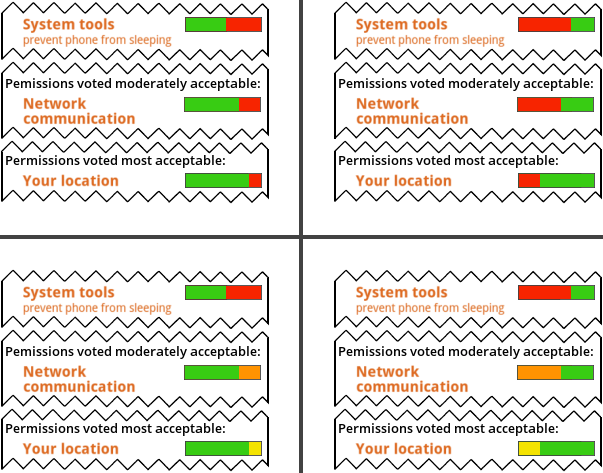
\includegraphics[width=.85\linewidth]{candidate-img/bars/barsR4.png}
%\end{center}
The first two interfaces used only red 
and green (with two variants: red on the left or red on the right),
so the goodness of a rating was indicated only by the ratio of red to green.
Unfortunately, subjects thought these bars were
progress bars or ratings of the 
permission's service quality.

The second two interfaces used red, orange, and yellow 
along with the green, so the goodness of the permission
was indicated both by the ratio of the warning color to green \emph{and} by the warning color
used. As with the red-green interfaces, one of the interfaces had the green on the left (so 
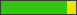
\includegraphics[height=8pt]{img/Bars4/RedYellowGreen/GreenYellowBar.png}\,,
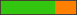
\includegraphics[height=8pt]{img/Bars4/RedYellowGreen/GreenOrangeBar.png}\,, and 
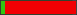
\includegraphics[height=8pt]{img/Bars4/RedYellowGreen/GreenRedBar.png}),
which I will call \emph{G-ROY} bars, and the
other had the warning color on the left (like 
\includegraphics[height=8pt]{img/Bars4/RedYellowGreen/YellowGreenBar.png}\,,
\includegraphics[height=8pt]{img/Bars4/RedYellowGreen/OrangeGreenBar.png}\,, and
\includegraphics[height=8pt]{img/Bars4/RedYellowGreen/RedGreenBar.png}),
which I will call \emph{ROY-G} bars.


Unlike the red-green only
bars, subjects still understood that the ratings were privacy related, and, 
unlike the warning-color only bars, 
they understood which ratings were better and which were worse. One subject
said of the orange bar that ``It means to me that feelings about 
this permission are mixed---about half of people think 
it is acceptable and half think it is not 
acceptable for this app to have that permission''. Thus I 
subjected these interfaces to large-scale testing (\refsec{s-sec-largescale}). 



\begin{wrapfigure}{l}{0.5\textwidth}
\begin{center}
\includegraphics[width=.9\linewidth]{candidate-img/traffic/trafficR2.png}
\end{center}
\end{wrapfigure}

\paragraph{Traffic Signs}
\label{s-sec-traffic}

The final set of interfaces I designed used traffic markers, 
an iconography suggested by a subject from another interface.
%``...a stop sign, caution sign, and a green light?''

\label{ss-sec-traffic-r2}
%\begin{center}
%\includegraphics[width=.5\linewidth]{candidate-img/traffic/trafficR2.png}
%\end{center}

The traffic marker interface split the permissions into three categories, with headers above
each category.
This interface successfully communicated that the ratings were related to privacy, 
but it exhibited a significant danger: the single green light gave subjects
the sense that all the permissions in the ``most acceptable'' category were 
completely safe and did
not need to be examined at all, which is not necessarily the
intended meaning. Additionally, this interface 
could be unsuitable for colorblind users.



\begin{wrapfigure}{r}{0.5\textwidth}
\begin{center}
\includegraphics[width=.9\linewidth]{candidate-img/traffic/trafficR3.png}
\end{center}
\end{wrapfigure}

To address colorblindness issues, I tried a variation using position
(as real traffic lights do). However, it still did not address
the problem of an overly-soothing green light. \\

%\label{ss-sec-traffic-r3}
%\begin{center}
%\includegraphics[width=.5\linewidth]{candidate-img/traffic/trafficR3.png}
%\end{center}


\begin{wrapfigure}{l}{0.5\textwidth}
\begin{center}
\includegraphics[width=.9\linewidth]{candidate-img/traffic/trafficR4.png}
\end{center}
\end{wrapfigure}


\label{ss-sec-traffic-r4}
%\begin{center}
%\includegraphics[width=.5\linewidth]{candidate-img/traffic/trafficR4.png}
%\end{center}

Rather than simply changing the colors of
the lights (which  
could look jarringly different from actual traffic lights and thus confuse users), 
the next interface used traffic \emph{signs}: a red octagon
(mimicking a stop sign), an orange diamond, and a yellow circle. 
Because the colors would be sparser in the interface (as they were only by the section 
headers) warning fatigue was less of
a concern than in the percentage bars 
(where they were next to every permission). 
As this interface was well understood by subjects so I included it
in the large-scale testing (\refsec{s-sec-largescale}).


\paragraph{Common Findings and Observations}
\label{common-findings}

These studies exposed two issues that arose in multiple 
interfaces. First, because Android is used in a range of 
cultures, some metaphors may not be familiar or applicable to all users.
For example, some countries 
do not use a letter grades in their schools.
Of my
interfaces, only the percentage bars do 
not rely on an existing metaphor and so avoid this particular confusion.

The second common issue was the better-or-worse phenomenon, 
wherein the more negative a rating is, the more positive subjects interpreted 
it to be. The net effect of this is alarming: The most dangerous permissions 
appear to be the most harmless! This problem is 
most troubling in the checkbox interface (\refsec{s-sec-checkbox}). 
There, dangerous permissions were indicated by a red X, but 
subjects thought the X meant that the permissions had been disabled, and therefore 
were \emph{completely innocuous}. Because of this phenomenon's dangerous nature, it greatly 
influenced my design decisions, and my selection of interfaces to study further.



\subsubsection{Interface Evaluation}
\label{s-sec-largescale}

Small-scale testing allowed me to eliminate all but three interfaces. 
To further validate these three, I carried out a large scale evaluation.

\paragraph{Methodology}
\label{subsec-large-methods}

As with the smaller studies, I posted surveys on Mechanical
Turk. I had 311 subjects for the traffic signs interface, 365
subjects for the G-ROY bar interface, and 83 subjects for the ROY-G bar
interface. The surveys explored four issues. 

Two are the same
as before: how well subjects understood the meaning of the interface
absent other cues, and whether subjects understood the ratings' source.
For these, I used the same prompts and mock-ups as for the
small-scale studies (\refsec{subsec-small-methods}).

In addition, I asked 
subjects how much they would trust ratings from each
of the three possible sources (``other Android users'', 
``independent security experts'', and ``a review team at Google''). 
For each source, subjects
had to select either ``I would not trust them at all'',
``I would trust them somewhat'', or ``I would trust 
them completely''.

Finally, I examined whether subjects would consider
these ratings useful for different types of users.
Specifically, I asked them to
provide ``yes''/``no'' answers for whether they would 
use such a system for themselves, recommend the system for use by a
parent (someone who might need assistance with technical decisions), and 
recommend it for use
by a teenager (someone for whom they might be
responsible).

\refsec{subsec-subject-understanding} will discuss how well
subjects understood the interface, \refsec{ssec-est-usage} will 
discuss the perception of utility of these ratings for different
populations, and \refsec{s-source} will discuss whether subjects 
understood the source of the ratings and how much they would trust each source.

\paragraph{The Purpose of the Ratings}
\label{subsec-subject-understanding}

I had two types of data to evaluate how well subjects understood
the meaning of the interface: text answers to the free-response 
question, and the Likert scale data.


% TODO: Add rubric back in
\begin{wrapfigure}{l}{0.6\textwidth}
\begin{center}
\includegraphics[width=.9\linewidth]{graphs/InterpPercentages.png}
    \caption{Percentage of subjects in each interpretation category.}
    \label{text-cat}
\end{center}
\end{wrapfigure}

To evaluate the text data, I, along with my advisor, manually coded  the correctness
of the interpretation of the interface for each of 
the responses.

To classify, we used a rubric that was revised until we obtained an
inter-coder reliability score ($\kappa$) of 0.835. 
The rubric is too large to reproduce here completely, but it has three
categories: \emph{Predominantly Correct Interpretation},
\emph{Semi-Correct Interpretation}, and \emph{Incorrect Interpretation}.
Fig.~\ref{text-cat} summarizes the percentages of subjects in
each class for each interface.




%\begin{wrapfigure}[r]{0.5\textwidth}
%\centering
%    \includegraphics[width=.5\linewidth]{graphs/InterpPercentages.png}
%    \caption{Percentage of subjects in each interpretation category.}
%    \label{text-cat}
%\end{wrapfigure}
Broadly classifying both correct and semi-correct
interpretations as understanding the interface,
all three interfaces had scores of over 50\%. 
The G-ROY bar interface had the lowest 
score, with 58\% of 
subjects having a correct or semi-correct interpretation. This is not significantly better 
than chance (Fisher's Exact test, $\mathrm{p}=0.053$). However, both the traffic 
sign interface and the ROY-G bar interface were 
significantly better than chance:
64\% (Fisher's Exact test, $\mathrm{p}<0.001$) for traffic signs and
66\% (Fisher's Exact test, $\mathrm{p}=0.04$) for the ROY-G bars. 

Note that these subjects had been given no explanation for the
interface, so these results represent a worst-case baseline. 
This would likely not occur in
the privacy-focused app store where users would have 
context for the ratings' meaning.

\begin{wrapfigure}{l}{0.65\textwidth}
\begin{center}
\includegraphics[width=.9\linewidth]{graphs/ClarityHistLikert.png}
    \caption{Subjects' responses to the Likert-type question asking users whether they thought it was clear that the icons represented privacy ratings.}
    \label{likert}\end{center}
\end{wrapfigure}

After subjects answered the free-response questions, I informed them that 
the icons were privacy ratings. I asked them to rate whether this was 
clear from the interface, on a 4-point Likert-type scale from ``completely 
unclear'' (a value of 1) to ``completely clear'' (a value of 4).
The ROY-G bars gave the best results, with a mean of 3.2.
However, both the G-ROY bars and the traffic signs also performed well,
with means of 2.9 and 3, respectively (shown in Fig.~\ref{likert}). 
In all three, the ratios of answers were 
significantly different from chance (using a $\chi$-squared test, all the interfaces had 
$\mathrm{p}< 0.05$).
%\begin{figure}[h]
%\centering
%    \includegraphics[width=.5\linewidth]{graphs/ClarityHistLikert.png}
%%    \caption{Subjects' responses to the Likert-type question asking users whether they thought it was clear that the icons represented privacy ratings.}
%    \label{likert}
%\end{figure}

\paragraph{Likelihood of Recommending the System}
\label{ssec-est-usage}

To determine if subjects felt the ratings would be useful for 
different audiences, I asked if 
they would personally use the ratings, and if
they would recommend them to a parent or
teenager. Subjects' responses did not 
differ significantly between interfaces, so I consider 
them in aggregate. Overall, 75\% of subjects said they would use the
ratings for themselves, 
74\% would use them for a teenager, and 72\% would use them for a parent. 
These results suggest there is a user base for these ratings.

\paragraph{The Source of Permission Ratings}
\label{s-source}

\begin{wrapfigure}{l}{0.65\textwidth}
\begin{center}
\includegraphics[width=.9\linewidth]{graphs/SourceBeliefs.png}
    \caption{Subjects' beliefs about the source of the ratings.}
    \label{src-beliefs}
    \end{center}
\end{wrapfigure}

As in the small-scale studies, I investigated whether subjects understood 
that the ratings were from other Android users. Subjects' beliefs are shown 
in Fig.~\ref{src-beliefs}.
During 
this large-scale study, a plurality of subjects understood that they were from other 
Android users, but there was still confusion. 
Although it would be ideal, it may not be possible to convey the 
source of the ratings solely through an interface. 

%\begin{figure}[ht]
%\centering
%    \includegraphics[width=.5\linewidth]{graphs/SourceBeliefs.png}
%%    \caption{Subjects' beliefs about the source of the ratings.}
%    \label{src-beliefs}
%\end{figure}

Over all, this study suggests that users are 
concerned about their privacy but currently lack the tools 
or expertise to control their own data and resources. My 
marketplace's privacy ratings of permissions provide users
with a mechanism to make informed decisions about apps.


%\section{Proposed Work}
%
%
%
%\subsection{Gathering User Ratings}
%\label{subsec-gather-ratings}
%
%\subsection{App Selection: Putting the Ratings to Work}
%\label{subsec-app-selection}
%
%\paragraph{Personalizing the Marketplace}
%\label{subsubsec-personalizing}
%
%
%
%\subsection{Analyzing Privacy Ratings}
%\label{subsec-analyzing-ratings}
%
%\subsubsection{The Effect of Branding}
%\label{subsubsec-branding}
%
%\subsubsection{Communicating With Developers}
%\label{subsubsec-dev-comm}
%
%\section{Evaluation}
%\label{sec-eval}
%
%\paragraph{Seeded User Ratings}
%
%\paragraph{The Apps}
%
%\paragraph{Analyzing Privacy Ratings}
%
%
%\section{Risks and Mitigations}
%
%\section{Future/Speculative Work}
%
%\paragraph{Paying for Privacy}
%
%\paragraph{The Permission Management Assistant}
%\label{subsubsec-perm-man-asst}


\section{Proposed Work}

I intend to gather user ratings of app permissions, create 
an app to present these ratings
to users (and obtain new ratings from them), and study factors that
affect how people perceive the reasonableness of permissions in
different apps. My primary means of disseminating ratings will be
an app that will use permission ratings as a means for sorting
apps (thereby giving priority to the least offensive apps). 
I discuss this app in Sec~\ref{subsec-the-apps}. 
In Sec~\ref{subsec-gather-ratings} 
I discuss my plans to obtain ratings at scale. In
Sec~\ref{subsec-app-selection} I talk about avenues for personalization 
and discuss how developers could use the permission ratings.

\subsection{The App}
\label{subsec-the-apps}

The primary goal of my proposed work is to give end users better tools to make decisions
about their privacy. I will do this directly by building an app, designed for the Android 
operating system, that can be installed 
and utilized by end users. (I will deploy the system as an app because 
apps are designed to be easy to install, so it will be available even to users 
with limited technical ability.) I choose to build atop Android for two reasons.
First, Android is a widely used operating system: according to Nielsen 
\cite{android-market-share}, a consumer research 
company, as of August, 2013, 52\% of smartphones in the United
States use Android, and its penetration in some other countries is
even higher.
Secondly, the Android permission model forces apps to explicitly state which permissions
they require to run, which allows me to programmatically extract the permissions for each 
app, making it much easier to evaluate the permissions. Additionally, 
since they have to approve the permissions of every app they install, 
most Android users have seen and interacted with permissions (even if they 
do not fully understand them).

\paragraph{A Privacy-Aware App Marketplace}
\label{subsubsec-privacy-store}

An app store offers users a way to search, examine, and download
apps.  Google Play, the built-in store for Android, gives
users access to over a million apps, and allows users to search by
popularity and functionality rating. Unfortunately, there is no way to incorporate
permission information in to the search. I believe this hinders the
user's ability to find privacy-conscious apps, because they have to
look at the permissions for each app they are considering, and are
heavily biased by the app \emph{quality} ratings (stars), which may
have little correlation with permission-sensitivity. My marketplace
will allow users to search by privacy criteria instead: in other
words, I will construct an app store that sorts apps primarily by
quality but secondarily by privacy-sensitivity, so that the best apps
\emph{that are also rated as requiring the most reasonable
  permissions} appear first.

Google Play does try to inform users about permissions by offering a
brief explanation of what each permission does. However, these
explanations are not specific to the app, and so do not help
users understand how the app might be using the permission. I 
believe this is an important factor, because in many cases a
permission that is perfectly legitimate for one app might be cause for
alarm in another. For example, location information makes 
sense for a weather app, but (absent other explanation) seems much
more suspicious for a flashlight app. In contrast, my app will
provide user ratings of each permission for each app 
as well as any responses or clarifications provided by the
developers. Because these ratings are specific to the app, I believe
they will enable users to arrive at a more \emph{informed} decision about
whether to install an app, given the permissions it requires.

Further highlighting the need for my type of marketplace, 
Felt et al.\ \cite{android-attention-SOUPS12} 
found that only 17\% of users surveyed looked at the permissions during
their last installation. The authors suggest that the timing of
permission presentation could contribute to the lack of attention paid
to the permissions, because it seems to encourage users to click
through the permissions to complete their task in much the same way
that pop-up warnings do. I believe that sorting apps by permissions
significantly ameliorates this problem, because sorting by permissions
means permissions have been significantly accounted for \emph{before}
users are required to make installation decisions.

To lift ratings from an individual permission to an entire app
requires some method of aggregation. I will design a
number of possible composition methods. One solution is to simply take
an average over the individual permission ratings. Other options would
be a sparklines-style composition where users could visually see the
general level approval of an apps permissions, or allowing the
community to rate the permissions that are most important for an app. 
Additionally, in 
Sec.~\ref{subsubsec-personalizing}, I propose that users
can establish personal privacy profiles, which would effectively offer
weights by which the permission ratings can be combined.

It should be noted here that regardless of whether users of the
marketplace are seeing ratings from Mechanical Turk workers or other
users, the app should make clear that these are community ratings, not
ratings provided by experts or the developers of the marketplace.


\subsection{Gathering User Ratings}
\label{subsec-gather-ratings}

Ideally, the users of my marketplace will provide ratings for
apps. However, 
to bootstrap the app, I will use Mechanical Turk to gather
ratings. In preliminary experiments, I found that I can obtain
quality ratings for no more than \$0.30 per worker. Since about thirty
ratings gives sufficiently strong reviews, I can rate each
app for no more than \$10. 
% TODO: Do I mention budget here?
My advisor and I have won a grant that  budgeted money to
seed the store with ratings, both for the most popular apps overall,
and for the most popular apps in select categories that people are
likely to search for (e.g., weather, finance, etc.).

This bootstrapping processes uses an ``offline'' model, in that I 
will accumulate these ratings so as to seed the marketplace before anyone
sees it. In principle, however, these ratings could also be done
``online'': that is, if a user is interested in a particular area, or
even a particular app, they could request ratings, spawning fresh tasks for
generating ratings on demand. 
%The speed at which a user gets reviews
%depends on number of variables, such as the time of day and day of
%week, but most importantly---based on my
%experiments---how much one is willing to pay for reviews. I 
%will post a series of tasks, staggered by time and
%cost, to construct an approximate valuation curve that indicates how
%much one needs to pay in return for obtaining quality reviews within a
%particular duration of time. In principle, this curve is a function
%that can be passed on to the user, who can decide how much they are
%willing to spend in return for how long they are willing to wait for
%reviews to be completed for their task.

In general, ratings will only be useful if they come from users with some
familiarity with the app models.
In my preparatory studies, I did not validate that respondents are
smartphone users (other than in the task description). In future
studies, I will ask users a test question such as what operating
system version they use on their device. Users could, of course, lie
about this, but it will help me to catch users who simply did not read
my task requirements.

\subsection{Putting the Ratings to Work}
\label{subsec-app-selection}

The permission ratings may be useful in helping users to choose apps, but
they could be used to improve the user's privacy in other ways as well. They could
also assist developers in understanding how users perceive their apps 
and improve their apps based on that feedback.

\paragraph{Personalizing the Marketplace}
\label{subsubsec-personalizing}

The privacy ratings are meant to help users make decision about whether
an app suits their specific privacy needs. Because each user will have a different
set of privacy concerns, the store would be more useful if it was personalized
to each user.

Building privacy profiles for each user would allow them to see ratings from
others with similar privacy mindsets, and to rank apps according to their
particular concerns. Privacy profiles could be built either by 
analyzing the reviews a user leaves, or by explicitly surveying them about their
privacy concerns. 

In addition to ratings from people with similar privacy philosophies, users may want to get
ratings from people they trust. Allowing people to build off of their existing 
social networks could give them greater confidence in the ratings. If users 
establish an account within the marketplace, they could designate other trusted
users, and choose to see reviews only from those users.
These other users could be trusted friends or family with stronger
computing or security knowledge (a stereotypical example of this is a
young adult helping their less comfortable parents or grandparents with technology).


\paragraph{Communicating With Developers}
\label{subsubsec-dev-comm}

The user ratings of app permissions will constitute a corpus of 
data about how users think about privacy, and how they use it to make decisions.
Thus far I have discussed how the ratings can be helpful to users, but
they can also be a valuable resource for developers. The ratings can tell
developers how users are perceiving their app and any trepidations users
have about the app's permissions. This could be addressed in one of two 
ways. If the app is over-privileged (it requests permissions it does not
use) or if the functionality using the permission is not necessary, the
permission could be removed, which may increase user confidence in the 
app. By examining how user opinion changes when permissions are changed,
developers can help balance their needs with those of their users. 

Alternatively, if a negatively-reviewed permission is necessary for
an app, the developers could still improve users' view of their app
if they explained to users \emph{why} the permission is required. In 
addition to helping users understand permissions, encouraging developers 
to clarify their permissions may establish a culture of communication
between users and developers. In a culture like this, an app that fails
to explain its permissions may raise red flags for users and cause them 
to be more cautious about 
installing it. 

Because developers will likely not be aware of my marketplace and 
consequently the permission ratings, they will not be able to respond 
to them. I will manually contact developers to call their attention
to the ratings and explain how they may be able to improve their 
app's image.


\section{Related Work}

Security and privacy in app systems is a multi-faceted issue, and 
so researchers have approached it from many angles.

Researchers such as \citet{99-problems-SPSM12} have found 
that smartphone users do take privacy risks seriously, but
\citet{smartphone-user-conf-SOUPS12} show that although
users are careful about
performing certain tasks on their phones, they engage in risky behavior
when it comes to installing apps. These
authors do not present solutions for users, but 
provide a foundation for my work.

There are several systems that offer additional 
security and privacy protections to Android users, such as 
\citet{mockDroid-HOTMOBILE11} and \citet{TISSA-Trust11}. 
These systems require modifying
the Android OS, which makes them impractical
for less technically adept users. 
\citet{dr-android-hide-SPSM12} also offer additional
protections, but require developers to rewrite their
apps to take advantage of them.
My interface is meant
for presenting additional information, and so could work
with the existing Android OS and apps, perhaps as a stand-alone app.

\citet{android-repackaged-CODASPY12} and others have
built systems that identify
malware. This is orthogonal to the scope of my work, which
deals with communicating the privacy risks of \emph{legitimate} apps.

There are also systems to detect misbehavior by apps (such as
\citet{taintDroid-OSDI10})
and others that use
automated methods to flag dangerous permissions (such as \citet{droidrisk-2013} 
and \citet{whyper-SEC13}). \citet{expect-purpose-UbiComp12}
use crowdsourcing to identify permissions that users do not expect,
and \citet{droidganger-SPSM12} use crowdsourcing to improve user 
understanding of Android permissions (although they are limited
to permissions that cause visual differences in app behavior). 
These works do not perform
extensive studies of \emph{interfaces to present} their output, which
is the focus of my work. In principle, their systems can be used to
generate the rating information that my interface provides.

\citet{nutrition-labels-SOUPS09} have also explored how to 
present privacy information to users.
They build off nutrition labels to develop a standardized 
presentation method for privacy policies, and found this 
display format helped users better understand the policy. 
Unfortunately, nutrition labels are not a good 
metaphor for user ratings because they imply an expert 
opinion. \citet{privacy-purchasing-effect-INFORMS11} 
show that when users look for products using a search engine 
annotated with privacy scores for the merchants, they are more 
likely to purchase products from sellers with higher privacy scores,
but they do not examine different interfaces for presenting
scores.


\section{Work Plan}

\begin{description}

\item[Summer 2015]
During this term I will design a method for aggregating 
permission-level ratings into an app-level rating. I will 
design several possible aggregation methods (such as a 
weighted average) and user test them on Mechanical
Turk to determine which is the most understandable and most
helpful to users. This will allow me to sort apps by their privacy 
rating as well as by their functionality rating.

I will also gather ratings for approximately 1000 apps to seed 
the marketplace (Sec~\ref{subsec-gather-ratings}). I will select these
apps by choosing the most popular apps in various categories on 
the Google Play store. I will extract the permission manifest and 
description for each app to build Mechanical Turk tasks. I will 
use these ratings from Mechanical Turk to populate a Postgres database 
for my app.

In addition to the Mechanical Turk ratings, I will also distribute
rating surveys to students on campus and computer security experts.
These surveys will provide me with a point of comparison against 
which to evaluate the Mechanical Turk ratings. 

\item[Fall 2015]

During this term I will gather ratings from automated sources 
such as Whyper~\cite{whyper-SEC13}, which finds permissions 
that are not explained by an app's description, and 
DroidRisk~\cite{droidrisk-2013}, which flags permissions or 
permissions combinations that are similar to those found in 
malware apps.

I will finish building the marketplace app. It 
will run on Android, and all the ratings and data for the apps in
the marketplace will be 
stored in the database, which will live on a Ruby server. The app 
will be released on the Play Store and available for download 
from my website. (My app will also be available for rating, 
and I will monitor any ratings we receive.)

I will perform usability studies to validate that users are able 
to understand and employ the app. These user studies will be posted
on Mechanical Turk, and run as in-person studies with participants
recruited on campus. If these studies reveal problems with the 
design of the app, I will incorporate that feedback into the app.

\item[Spring 2016] 
During this semester I will examine the app ratings, and determine 
cases where developers might be able to adjust their permissions
or provide better explanations to address user concerns. I will 
reach out to app developers to discuss how they could make their 
apps meet their users' privacy needs or clarify their permission 
requirements (Sec~\ref{subsubsec-dev-comm}). 
This will entail calling attention to the way users are perceiving 
their app's permissions, and possibly providing feedback on how
to address user concerns.

\end{description}

\singlespacing




%\section{Personnel and Work Plan}
%
%
%
%\paragraph{Dissemination Plan}
%
%The proposal's goal is to produce not only designs but also working
%software artifacts. The PI has a strong track record in this regard:
%he has led the design and deployment of DrRacket and WeScheme
%(programming environments), FrTime and Flapjax (programming
%languages), Margrave (policy analyzer), $\lambda_{JS}$ (semantics for
%JavaScript), TeJaS (type system for JavaScript), Continue (conference
%manager), and more.
%
%We intend to continue to influence both research and practice by
%disseminating robust systems. All code will be released with the most
%generous licenses---ideally Open Source---permitted by the components we
%build on. We are also experienced in building and nurturing user
%communities for my systems.
%
%\paragraph{Work Plan}
%
%The project will be executed primarily by the PhD student in
%conjunction with the PI. However, we also expect to include several
%undergraduates in the work. Indeed, the graduate student already has
%experience shepherding undergraduate collaborators to a published
%research paper \cite{usable-sec-analysis-ONWARD13}. We anticipate the 
%years being divided as
%follows:
%\begin{description}
%
%\item[Year 1]
%During the first year we will complete studies on the user interface design
%(Sec~\ref{subsec-perm-ui}). This will allow us to build prototypes of the 
%apps for testing (Sec~\ref{subsec-the-apps}). These prototype apps will 
%also be completed in the first year. We will also gather ratings for approximately 1000 
%apps to seed my prototype (Sec~\ref{subsec-gather-ratings}). This will be 
%necessary to perform realistic user studies.
%% Some studies and a first prototype
%
%\item[Year 2]
%During the second year we will complete those studies that depend on the 
%prototype apps, such as examining how users decide their priorities
%in the trade off between functionality and privacy (Sec~\ref{subsec-analyzing-ratings}). We will use the results of these
%studies to design features for my apps that are meant to encourage
%secure behavior in users (Sec~\ref{subsec-app-selection}).
%% Further studies that depend on the prototype
%
%\item[Year 3]
%During this year, we will rebuild my apps to incorporate the 
%features designed in year two, to allow users to personalize the app store 
%and expand communication channels between users and developers 
%(Sec~\ref{subsec-app-selection}).
%
%We will also redesign my original studies for other platforms that
%are popular at the time, such as (potentially) Windows, Firefox OS, etc.
%% Expanding prototypes in to more robust apps. Repeating studies 
%% on other platforms.
%
%\end{description}
%
%
%\section{Broader Impact}
%
%my proposal is driven heavily by its intended social impact on
%non-technical end-users. App stores have become my most standard
%app delivery platform, and their success means they are
%expanding into ever more domains. Simply by virtue of their widespread
%use, which is starting to encompass a notable percentage of the
%Earth's population, most of their users are necessarily not technical
%or security experts. At the same time, apps are starting to
%penetrate more and more private aspects of peoples' lives. As a
%result, techniques to improve the privacy-relevant decisions of users
%are of pressing and urgent need.
%
%In this area, my work is focusing on user-facing areas. We are
%studying user perceptions of ratings and of interface choices. All
%these are meant to directly assist end-users in employing the results
%of this work.



\newpage
\hypersetup{pageanchor=false}
\setcounter{page}{1}

\bibliographystyle{terseabbrvnat}
\renewenvironment{FlushLeft}{}{}
%\bibliography{../NSF-2011/safebrowser,shriram}
\bibliography{proposal}


\newpage
\pagestyle{empty}
\hypersetup{pageanchor=false}
\setcounter{page}{1}

\end{document}
